\documentclass[12pt,a4paper]{article}
\usepackage[a4paper,margin=1in]{geometry}
\usepackage{graphicx}
\usepackage{booktabs}
\usepackage{longtable}
\usepackage{array}
\usepackage{float}
\usepackage{caption}
\usepackage{subcaption}
\usepackage{amsmath}
\usepackage{hyperref}
\usepackage{setspace}
\usepackage{enumitem}
\usepackage{titlesec}

\graphicspath{{ns-allinone-3.39/ns-3.39/graphs/}}
\hypersetup{colorlinks=true,linkcolor=black,urlcolor=blue,citecolor=black}
\onehalfspacing
\setlength{\parskip}{0.5em}
\setlength{\parindent}{0pt}
\titleformat{\section}{\large\bfseries}{\thesection.}{0.5em}{}
\titleformat{\subsection}{\normalsize\bfseries}{\thesubsection}{0.5em}{}

\begin{document}

\begin{titlepage}
\centering
{\Large Bangladesh University of Engineering and Technology (BUET) \par}
\vspace{1.5cm}
{\LARGE \textbf{Simulation Report}}\par
\vspace{0.4cm}
{\Large \textbf{FF-AODV: Energy and Velocity Aware Routing in ns-3.39}}\par
\vspace{1.2cm}

\begin{tabular}{ll}
\textbf{Course:} & CSE 322 -- Computer Networks Sessional \\
\textbf{Topic:} & Routing protocol modification and performance evaluation \\
\textbf{Simulator:} & ns-3.39 (C++) \\
\textbf{Author:} & Mosharaf Hossain Apurbo \\
\textbf{Date:} & April 8, 2026
\end{tabular}

\vfill
\textbf{Abstract}
\end{titlepage}

\section*{Abstract}
This report presents a complete ns-3.39 based simulation study of a modified AODV protocol named FF-AODV (Fitness Function AODV). The assignment-required static topologies are covered using (i) IEEE 802.11b ad-hoc and (ii) an IEEE 802.15.4-like emulation setup. A bonus mobile FANET scenario is additionally evaluated using IEEE 802.11a with Gauss-Markov mobility. The protocol is implemented in two phases: Phase 1 (energy + hop aware) and Phase 2 (energy + hop + velocity aware). The report includes topology descriptions, parameter variations, exact simulator-level changes, results with graphs, summary findings, and reflection/discussion. Results show expected degradation under larger areas and higher offered load, while the Phase 2 mobility-aware extension provides only modest changes over Phase 1 in the currently available speed-sweep dataset, indicating that higher statistical repetition and broader stress conditions are needed for stronger conclusions.

\tableofcontents
\newpage

\section{Introduction}
Standard AODV prioritizes route discovery and freshness but fundamentally prefers routes by sequence number and hop count related logic. In mobile and energy constrained wireless settings, this can be suboptimal because:
\begin{enumerate}[leftmargin=1.5em]
    \item low-energy relays can be repeatedly overused,
    \item high-speed relays can destabilize routes,
    \item shortest path alone does not capture route robustness.
\end{enumerate}

To address this, FF-AODV introduces a fitness score that combines residual energy, path efficiency, and in Phase 2, velocity stability. The main goals of this report are:
\begin{enumerate}[leftmargin=1.5em]
    \item present all assignment-required simulation topologies and parameter sweeps,
    \item document simulator code modifications in detail,
    \item analyze result trends using generated graphs and CSV values,
    \item summarize findings and discuss limitations and future improvements.
\end{enumerate}

\section{Network Topologies Under Simulation}

\subsection{Topology A: Wireless 802.11 Static}
This topology uses the program \texttt{scratch/sim-802-11-static.cc}. Key characteristics are:
\begin{itemize}[leftmargin=1.5em]
    \item Standard: IEEE 802.11b ad-hoc (DSSS 1 Mbps fixed rate).
    \item Mobility: static nodes (\texttt{ConstantPositionMobilityModel}).
    \item Placement: random uniform in square area of side $\text{areaFactor} \times \text{txRange}$.
    \item Traffic: UDP OnOff, packet size 512 bytes.
    \item Energy: \texttt{BasicEnergySource} (100 J) + \texttt{WifiRadioEnergyModel}.
    \item Routing settings (Phase 1 mode): $\alpha=0.6$, $\beta=0.4$, $\gamma=0.0$.
\end{itemize}

\subsection{Topology B: 802.15.4-like Static Emulation}
This topology uses \texttt{scratch/sim-802-15-4-static.cc}. It is intentionally configured to emulate low-rate, short-range behavior:
\begin{itemize}[leftmargin=1.5em]
    \item PHY/MAC base: 802.11b ad-hoc with reduced Tx power (9 dBm).
    \item Emulation intent: short range and small payload behavior similar to 802.15.4.
    \item Packet size: 80 bytes (close to practical 802.15.4 payload limits).
    \item Area base: \texttt{txRange=50 m} (smaller than 802.11 setup).
    \item Mobility: static.
    \item Routing settings: $\alpha=0.6$, $\beta=0.4$, $\gamma=0.0$.
\end{itemize}

\textbf{Important implementation note:} true IPv4 + AODV over LR-WPAN + 6LoWPAN is stated in code comments as problematic for this setup in ns-3.39, hence this controlled emulation was used.

\subsection{Topology C (Bonus): FANET Mobile Scenario}
Two scripts are used for comparison:
\begin{itemize}[leftmargin=1.5em]
    \item \texttt{scratch/sim-fanet-phase1-bonus.cc} (Phase 1 baseline),
    \item \texttt{scratch/sim-fanet-bonus.cc} (Phase 2 velocity-aware).
\end{itemize}

Common FANET settings:
\begin{itemize}[leftmargin=1.5em]
    \item Standard: 802.11a ad-hoc at 6 Mbps.
    \item Mobility: \texttt{GaussMarkovMobilityModel} in 3D bounds $500\times500\times100$.
    \item Energy: 100 J per node with WiFi radio model.
    \item Traffic: UDP OnOff, packet size 512 bytes.
    \item Variable of interest: node speed (5, 10, 15, 20, 25 m/s).
\end{itemize}

\section{Parameters Under Variation}

\subsection{Assignment-Aligned Parameter Sweeps}
The mandatory static study varied one parameter at a time while keeping others fixed.

\begin{table}[H]
\centering
\caption{Parameter values used in the sweeps}
\begin{tabular}{ll}
\toprule
\textbf{Parameter} & \textbf{Values} \\
\midrule
Number of nodes & 20, 40, 60, 80, 100 \\
Number of flows & 10, 20, 30, 40, 50 \\
Packets per second & 100, 200, 300, 400, 500 \\
Coverage area factor (static) & 1, 2, 3, 4, 5 \\
Node speed (mobile bonus) & 5, 10, 15, 20, 25 m/s \\
\bottomrule
\end{tabular}
\end{table}

\subsection{Fixed Baselines per Sweep}
From the automation scripts:
\begin{itemize}[leftmargin=1.5em]
    \item Static defaults: $nNodes=40$, $nFlows=10$, $pktPerSec=100$, $areaFactor=1$.
    \item FANET phase-comparison defaults: $nNodes=60$, $nFlows=15$, $pktPerSec=20$, multi-seed runs.
\end{itemize}

\subsection{Measured Metrics}
All required metrics are captured:
\begin{enumerate}[leftmargin=1.5em]
    \item Network throughput (Mbps)
    \item Average end-to-end delay (ms)
    \item Packet delivery ratio (PDR, \%)
    \item Packet drop ratio (PDrop, \%)
    \item Total energy consumption (J)
\end{enumerate}

\section{Modifications Made in the Simulator}

\subsection{Fitness Function Design}
\subsubsection*{Phase 1 (Energy + Hop)}
\begin{equation}
F_{p1} = \alpha \cdot \frac{E_{res}}{E_{init}} + \beta \cdot \frac{1}{h}
\end{equation}
where $\alpha=0.6$, $\beta=0.4$ in static experiments.

\subsubsection*{Phase 2 (Energy + Hop + Velocity)}
\begin{equation}
F_{p2} = \alpha \cdot \frac{E_{res}}{E_{init}} + \beta \cdot \frac{1}{h} + \gamma \cdot \frac{V_{max}-V}{V_{max}}
\end{equation}
with Phase 2 defaults: $\alpha=0.5$, $\beta=0.3$, $\gamma=0.2$, $V_{max}=50$ m/s.

The path fitness is propagated using a weakest-link principle:
\begin{equation}
F_{path} = \min(F_{incoming}, F_{local})
\end{equation}
and the path velocity field tracks worst-case mobility:
\begin{equation}
V_{path} = \max(V_{incoming}, V_{local})
\end{equation}

\subsection{AODV Data Structure and Packet-Level Changes}
The following simulator-level changes were made inside \texttt{src/aodv}:
\begin{itemize}[leftmargin=1.5em]
    \item Added path fitness and velocity fields to RREQ and RREP headers.
    \item Extended (de)serialization for both fields:
    \begin{itemize}[leftmargin=2em]
        \item RREQ size became 39 bytes (23 + 8 + 8).
        \item RREP size became 35 bytes (19 + 8 + 8).
    \end{itemize}
    \item Added route-entry fitness field in routing table entries.
\end{itemize}

\subsection{Routing Decision Logic Changes}
Core behavioral changes in routing protocol implementation include:
\begin{enumerate}[leftmargin=1.5em]
    \item Reverse-route updates in RREQ processing use fitness comparison.
    \item Duplicate RREQ handling is relaxed: duplicates are accepted only if fitness improves.
    \item RREP path fitness/velocity are seeded and propagated so destination-side contribution is preserved.
    \item When sequence numbers tie in RREP update logic, route preference is based on better fitness (instead of hop-only preference).
\end{enumerate}

\subsection{Build Integration}
The AODV module build now links with energy library support (\texttt{\${libenergy}}) in \texttt{src/aodv/CMakeLists.txt} to enable direct residual-energy access in routing logic.

\subsection{Files Modified (Summary)}
\begin{longtable}{p{0.34\textwidth}p{0.6\textwidth}}
\toprule
\textbf{File} & \textbf{Main Modification} \\
\midrule
\endhead
\texttt{src/aodv/model/aodv-packet.h} & Added fitness and velocity fields with getters/setters in RREQ and RREP headers. \\
\texttt{src/aodv/model/aodv-packet.cc} & Serialization/deserialization updates for new fields; updated header sizes and print/equality behavior. \\
\texttt{src/aodv/model/aodv-rtable.h} & Added route fitness member and accessor methods. \\
\texttt{src/aodv/model/aodv-rtable.cc} & Initialized route fitness default to 0.0. \\
\texttt{src/aodv/model/aodv-routing-protocol.h} & Added velocity-related parameters and updated fitness function signature. \\
\texttt{src/aodv/model/aodv-routing-protocol.cc} & Implemented fitness calculation, energy and mobility extraction, RREQ/RREP propagation and update rules. \\
\texttt{src/aodv/CMakeLists.txt} & Linked energy library dependency. \\
\bottomrule
\end{longtable}

\section{Results With Graphs}

\subsection{Overview Graphs (Mandatory Static Study)}
The following all-metric dashboards aggregate throughput, delay, PDR, drop ratio, and energy for each variation axis.

\begin{figure}[H]
\centering
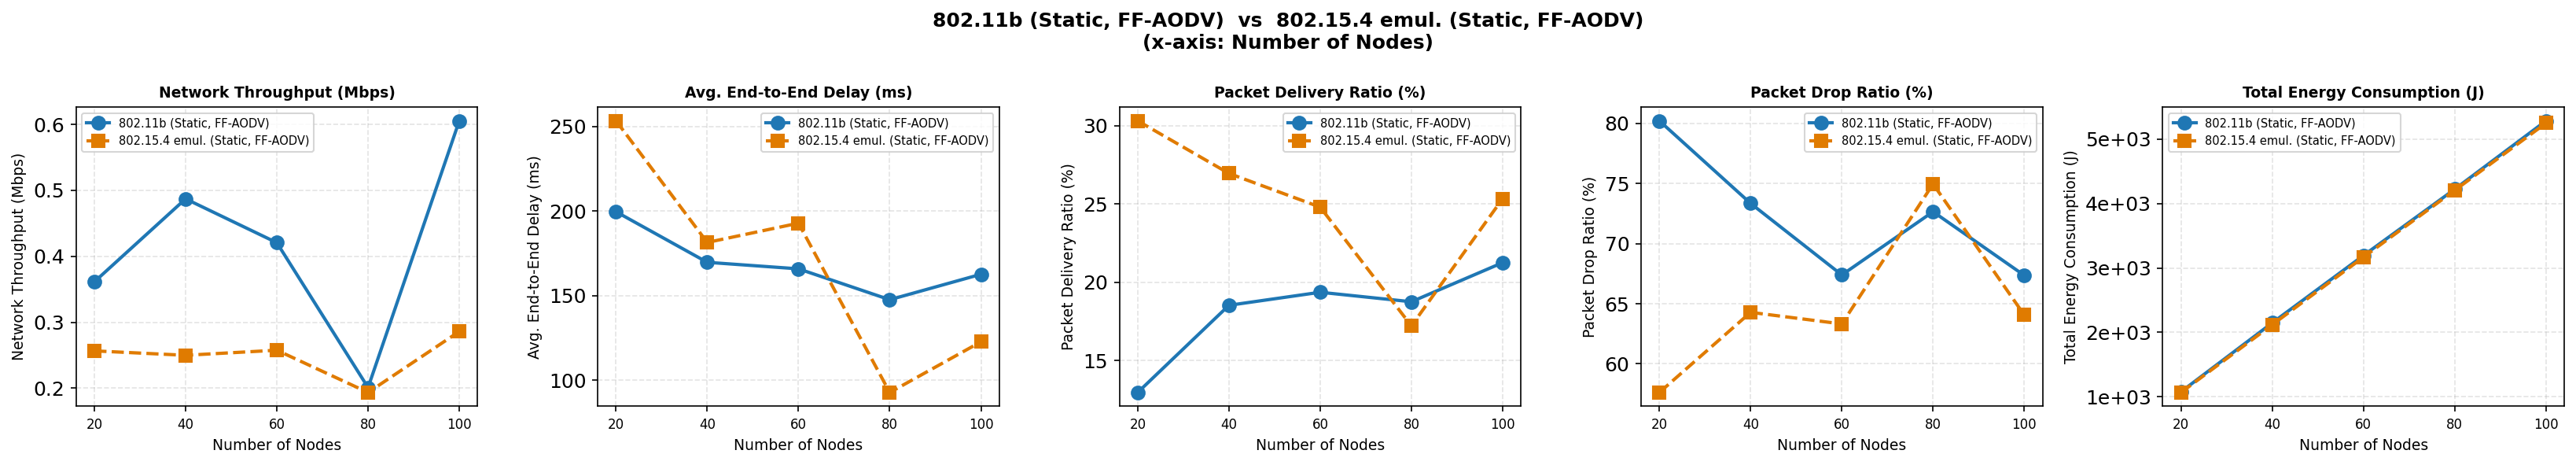
\includegraphics[width=0.9\textwidth]{overview/compare_vary_nodes_all_metrics.png}
\caption{802.11 vs 802.15.4-like emulation: all metrics while varying number of nodes}
\end{figure}

\begin{figure}[H]
\centering
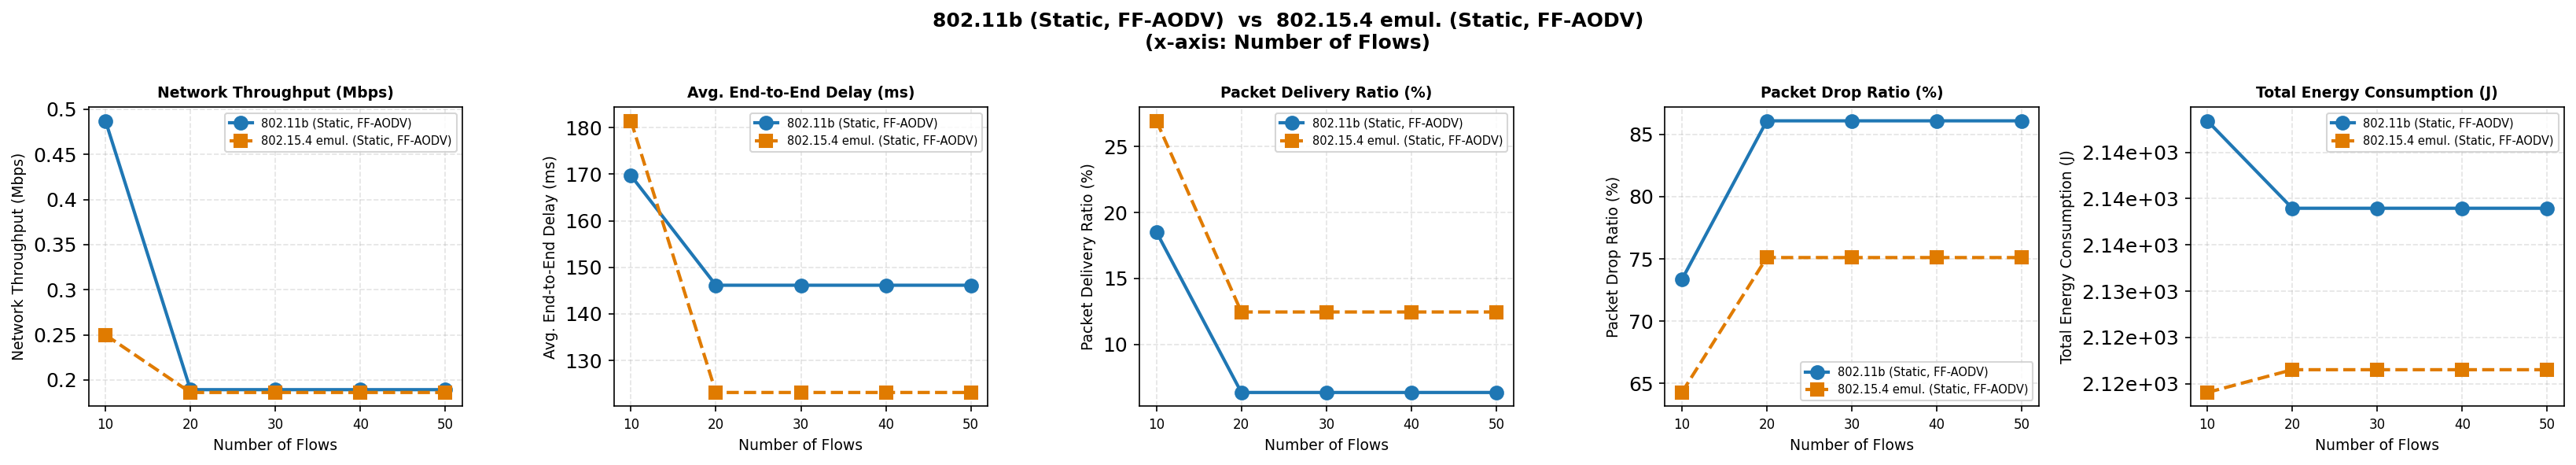
\includegraphics[width=0.9\textwidth]{overview/compare_vary_flows_all_metrics.png}
\caption{802.11 vs 802.15.4-like emulation: all metrics while varying number of flows}
\end{figure}

\begin{figure}[H]
\centering
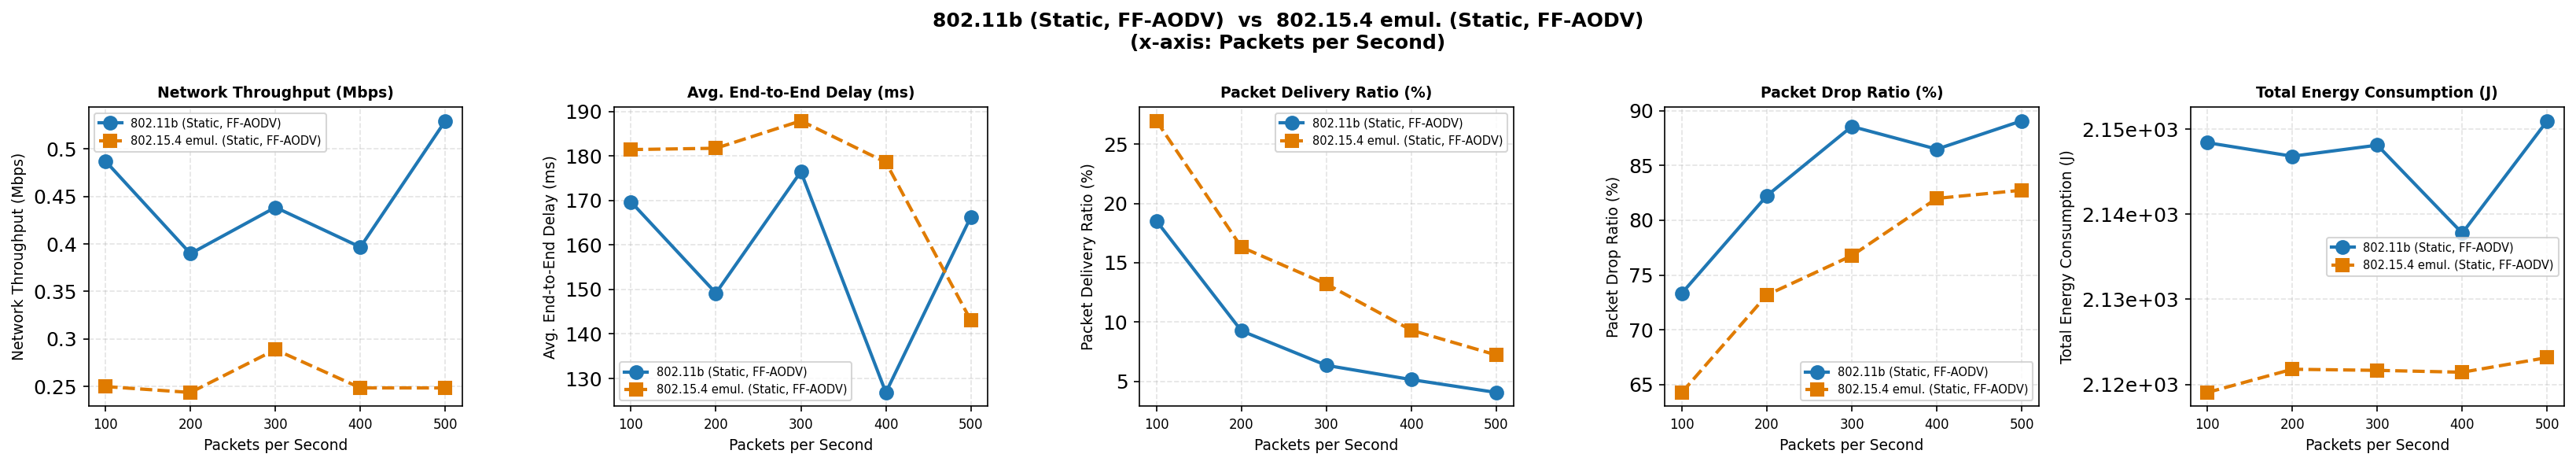
\includegraphics[width=0.9\textwidth]{overview/compare_vary_pps_all_metrics.png}
\caption{802.11 vs 802.15.4-like emulation: all metrics while varying packet rate}
\end{figure}

\begin{figure}[H]
\centering
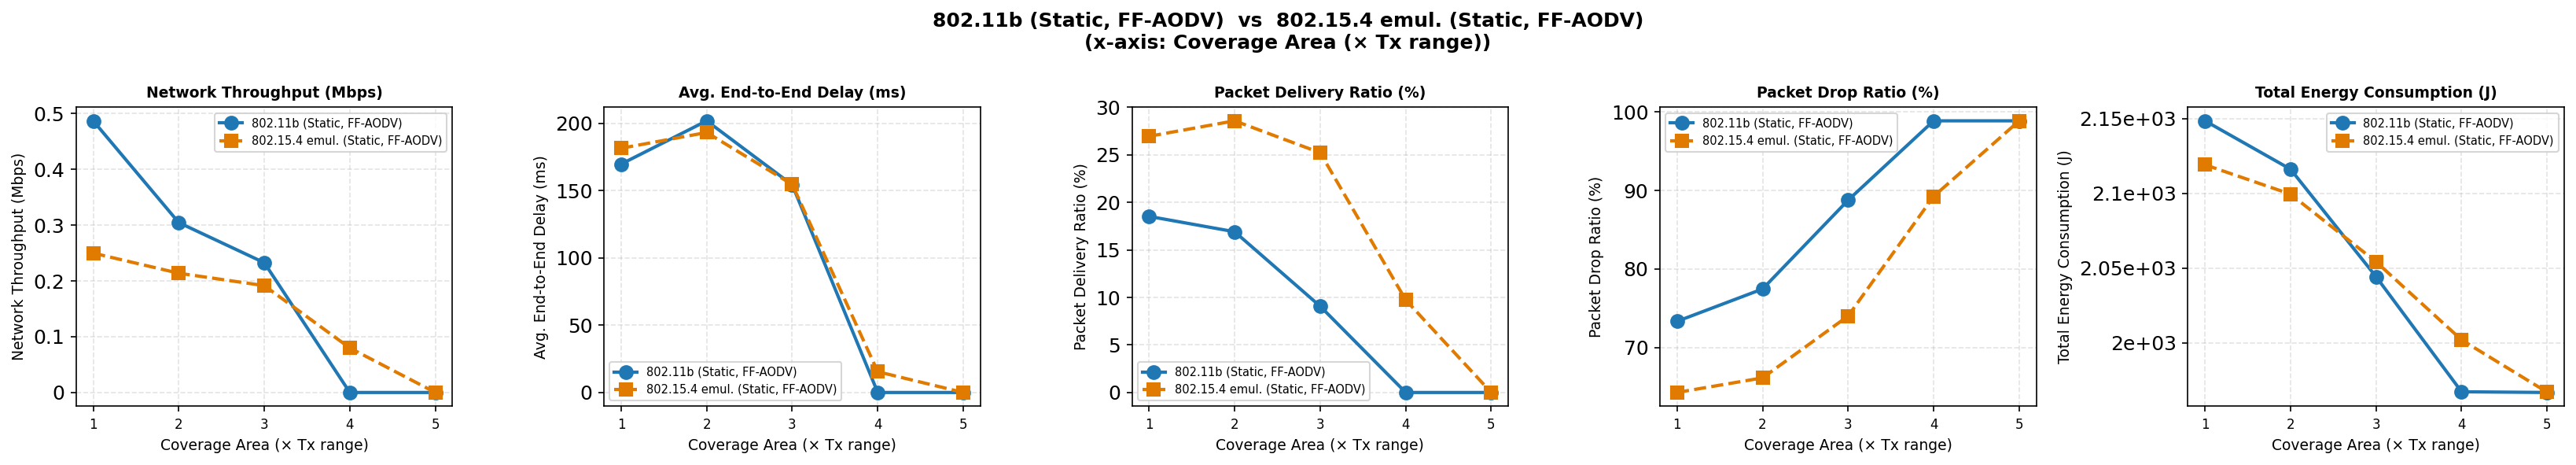
\includegraphics[width=0.9\textwidth]{overview/compare_vary_area_all_metrics.png}
\caption{802.11 vs 802.15.4-like emulation: all metrics while varying coverage area}
\end{figure}

\subsection{Numerical Results: Static Topologies}

\subsubsection*{A. Varying Number of Nodes}
\begin{table}[H]
\centering
\scriptsize
\caption{Node sweep results (static, area factor=1, flows=10, pps=100)}
\begin{tabular}{rrrrrrrrr}
\toprule
Nodes & T11 & T154 & D11 & D154 & PDR11 & PDR154 & Drop11 & Drop154 \\
\midrule
20  & 0.361 & 0.257 & 199.618 & 253.406 & 12.955 & 30.321 & 80.207 & 57.623 \\
40  & 0.487 & 0.250 & 169.697 & 181.450 & 18.528 & 26.959 & 73.344 & 64.285 \\
60  & 0.421 & 0.258 & 165.836 & 192.851 & 19.361 & 24.804 & 67.394 & 63.322 \\
80  & 0.201 & 0.193 & 147.577 & 92.692  & 18.755 & 17.212 & 72.652 & 74.957 \\
100 & 0.605 & 0.286 & 162.614 & 122.674 & 21.254 & 25.343 & 67.354 & 64.058 \\
\bottomrule
\end{tabular}
\end{table}

\textbf{Observation:}
Throughput is generally higher in 802.11. Both systems show non-monotonic behavior due random placement and single-run per point in static sweeps. Energy consumption (not shown in this compact table) grows with node count in both systems, reaching about 5281 J (802.11) and 5246 J (802.15.4-like) at 100 nodes.

\subsubsection*{B. Varying Number of Flows}
\begin{table}[H]
\centering
\scriptsize
\caption{Flow sweep results (static, nodes=40, area factor=1, pps=100)}
\begin{tabular}{rrrrrrrrr}
\toprule
Flows & T11 & T154 & D11 & D154 & PDR11 & PDR154 & Drop11 & Drop154 \\
\midrule
10 & 0.487 & 0.250 & 169.697 & 181.450 & 18.528 & 26.959 & 73.344 & 64.285 \\
20 & 0.189 & 0.186 & 146.149 & 123.123 & 6.346  & 12.453 & 86.087 & 75.114 \\
30 & 0.189 & 0.186 & 146.149 & 123.123 & 6.346  & 12.453 & 86.087 & 75.114 \\
40 & 0.189 & 0.186 & 146.149 & 123.123 & 6.346  & 12.453 & 86.087 & 75.114 \\
50 & 0.189 & 0.186 & 146.149 & 123.123 & 6.346  & 12.453 & 86.087 & 75.114 \\
\bottomrule
\end{tabular}
\end{table}

\textbf{Observation:}
The flat values from 20 to 50 flows are a direct artifact of implementation capping: \texttt{actualFlows = min(nFlows, nNodes/2)}. With $nNodes=40$, the effective maximum is 20 flows, so requested values above 20 do not create additional offered load.

\subsubsection*{C. Varying Packets per Second}
\begin{table}[H]
\centering
\scriptsize
\caption{Packet-rate sweep results (static, nodes=40, flows=10, area factor=1)}
\begin{tabular}{rrrrrrrrr}
\toprule
PPS & T11 & T154 & D11 & D154 & PDR11 & PDR154 & Drop11 & Drop154 \\
\midrule
100 & 0.487 & 0.250 & 169.697 & 181.450 & 18.528 & 26.959 & 73.344 & 64.285 \\
200 & 0.390 & 0.244 & 149.182 & 181.747 & 9.266  & 16.321 & 82.233 & 73.176 \\
300 & 0.439 & 0.289 & 176.482 & 187.912 & 6.358  & 13.209 & 88.558 & 76.769 \\
400 & 0.397 & 0.248 & 126.850 & 178.586 & 5.156  & 9.321  & 86.485 & 81.994 \\
500 & 0.530 & 0.248 & 166.312 & 143.060 & 4.072  & 7.231  & 89.071 & 82.738 \\
\bottomrule
\end{tabular}
\end{table}

\textbf{Observation:}
Both systems suffer PDR reduction and drop-ratio increase with rising offered packet rate. 802.11 maintains higher throughput envelope, while 802.15.4-like stays lower and more constrained.

\subsubsection*{D. Varying Coverage Area}
\begin{table}[H]
\centering
\scriptsize
\caption{Area sweep results (static, nodes=40, flows=10, pps=100)}
\begin{tabular}{rrrrrrrrr}
\toprule
AreaF & T11 & T154 & D11 & D154 & PDR11 & PDR154 & Drop11 & Drop154 \\
\midrule
1 & 0.487 & 0.250 & 169.697 & 181.450 & 18.528 & 26.959 & 73.344 & 64.285 \\
2 & 0.305 & 0.214 & 201.835 & 193.172 & 16.914 & 28.585 & 77.464 & 66.145 \\
3 & 0.233 & 0.192 & 154.255 & 154.538 & 9.076  & 25.230 & 88.769 & 74.021 \\
4 & 0.000 & 0.080 & 0.000   & 15.424  & 0.000  & 9.738  & 98.877 & 89.252 \\
5 & 0.000 & 0.000 & 0.000   & 0.000   & 0.000  & 0.000  & 98.877 & 98.877 \\
\bottomrule
\end{tabular}
\end{table}

\textbf{Observation:}
Area expansion strongly harms connectivity. At larger area factors, both networks approach near-disconnection behavior (very low throughput and near-total packet loss).

\subsection{Bonus Results: FANET Phase 1 vs Phase 2}

\begin{figure}[H]
\centering
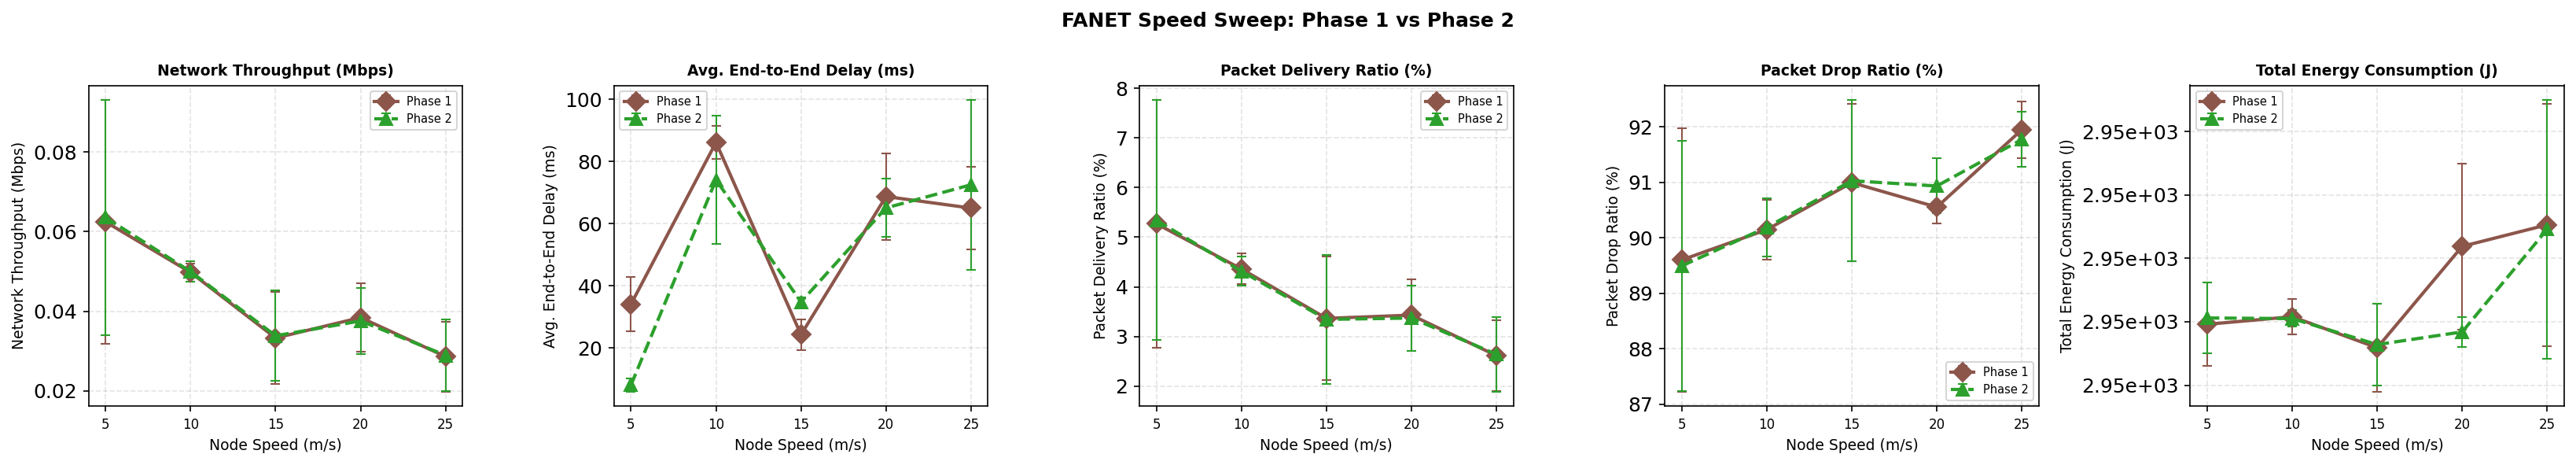
\includegraphics[width=0.9\textwidth]{overview/fanet_phase1_vs_phase2_all_metrics.png}
\caption{FANET comparison dashboard: Phase 1 (energy+hop) vs Phase 2 (energy+hop+velocity)}
\end{figure}

\begin{figure}[H]
\centering
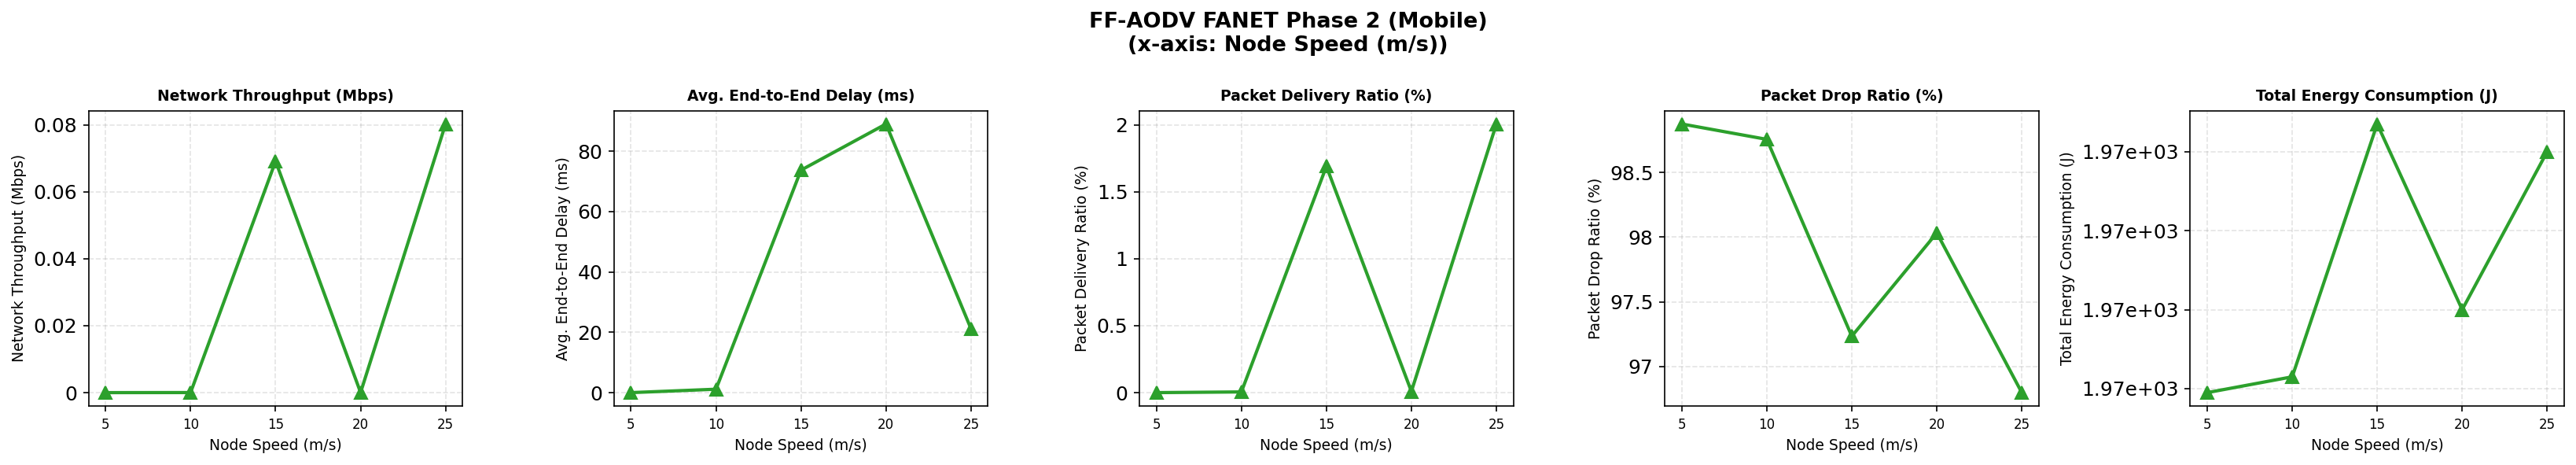
\includegraphics[width=0.9\textwidth]{overview/fanet_vary_speed_all_metrics.png}
\caption{FANET Phase 2 speed-sweep overview}
\end{figure}

\begin{table}[H]
\centering
\scriptsize
\caption{Mean FANET metrics by speed (current available runs)}
\begin{tabular}{rrrrrrr}
\toprule
Speed & T(P1) & T(P2) & Delay(P1) & Delay(P2) & PDR(P1) & PDR(P2) \\
(m/s) & Mbps & Mbps & ms & ms & \% & \% \\
\midrule
5  & 0.062442 & 0.063529 & 34.074 & 8.076  & 5.271 & 5.342 \\
10 & 0.049755 & 0.049951 & 86.100 & 74.040 & 4.361 & 4.315 \\
15 & 0.033288 & 0.033839 & 24.264 & 34.786 & 3.365 & 3.345 \\
20 & 0.038421 & 0.037574 & 68.691 & 65.022 & 3.431 & 3.372 \\
25 & 0.028615 & 0.028945 & 64.974 & 72.468 & 2.616 & 2.641 \\
\bottomrule
\end{tabular}
\end{table}

\textbf{Observation:}
In the present dataset, Phase 2 and Phase 1 are very close in throughput and PDR across speeds, with mixed delay differences. This indicates modest net effect under the chosen stress level and sample count, not a clear universal gain or loss.

\section{Summary Findings}

\begin{enumerate}[leftmargin=1.5em]
    \item \textbf{Topology behavior:} Both static topologies degrade with higher area and traffic stress; 802.11 generally provides higher throughput than the 802.15.4-like emulation.
    \item \textbf{Connectivity sensitivity:} Coverage-area increase is the strongest stress factor; both topologies approach near-total drop around the highest area factors.
    \item \textbf{Protocol modification correctness:} FF-AODV fitness propagation is integrated consistently into RREQ/RREP logic, route-table storage, and tie-break route updates.
    \item \textbf{Bonus mobility comparison:} Phase 2 velocity-aware routing currently shows small, mixed differences versus Phase 1 in available mean results.
    \item \textbf{Energy trend:} Total consumed energy increases with network size/load as expected; mobility-phase comparison shows only minor energy differences between phases.
\end{enumerate}

\section{Reflection and Discussion}

\subsection{What Worked Well}
\begin{itemize}[leftmargin=1.5em]
    \item The simulator modifications are deep (packet format, routing table, route-update logic) and therefore academically meaningful.
    \item The full automation pipeline (simulation + plotting) improves reproducibility and minimizes manual reporting error.
    \item Weakest-link path fitness and worst-case path velocity are conceptually aligned with stability-aware routing.
\end{itemize}

\subsection{Important Limitations in Current Results}
\begin{enumerate}[leftmargin=1.5em]
    \item \textbf{Flow-sweep capping artifact:} in static scripts, effective flow count is capped at $nNodes/2$; therefore requested flows above 20 (for $nNodes=40$) do not actually increase offered load.
    \item \textbf{Single-run static points:} non-monotonic curves are expected when each point has only one random realization.
    \item \textbf{802.15.4 representation:} this is an emulation through tuned WiFi behavior, not a full LR-WPAN + IPv6 routing stack experiment.
    \item \textbf{FANET sample depth:} current available phase-comparison CSV has limited run count, so confidence intervals are not yet tight.
\end{enumerate}

\subsection{Interpretation of Phase 2 Outcome}
The velocity-aware term does not guarantee universal improvement in every metric at every speed. This is expected in MANET/FANET studies where route quality, contention, and mobility interact nonlinearly. A robust claim requires more seeds and scenario diversity.

\subsection{Recommended Next Steps}
\begin{enumerate}[leftmargin=1.5em]
    \item Remove or parameterize the flow capping effect for true 10--50 flow stress tests.
    \item Run 5--10 seeds for all static points and report mean with variance bars.
    \item Add confidence intervals for FANET Phase 1 vs Phase 2.
    \item Evaluate additional mobility models and larger offered loads.
\end{enumerate}

\section{Reproducibility Commands}
All results and graphs in this project are generated from scripts in \texttt{ns-allinone-3.39/ns-3.39}.

\begin{verbatim}
# From ns-allinone-3.39/ns-3.39
./run_all_simulations.sh
./run_fanet_phase_comparison.sh
python3 plot_graphs.py
python3 plot_fanet_phase_comparison.py
\end{verbatim}

\section{Conclusion}
This work successfully implements and evaluates FF-AODV in ns-3.39 with assignment-compliant static experiments and a mobility-aware FANET extension. The report demonstrates end-to-end protocol engineering: metric design, packet/routing state extensions, routing-decision rewrites, experiment automation, and graph-backed analysis. The most impactful practical insight is that methodological details (effective load, random-seed count, and topology realism) strongly influence interpretation; therefore, simulator modifications and experimental design must be validated together for defensible conclusions.

\section*{References}
\begin{enumerate}[leftmargin=1.5em]
    \item A. Taha et al., ``Energy Efficient Multipath Routing Protocol for Mobile Ad-Hoc Network Using the Fitness Function,'' \textit{IEEE Access}, vol. 5, 2017.
    \item ns-3 Consortium, ``ns-3 Network Simulator,'' \url{https://www.nsnam.org/}.
    \item Project scripts and source code in this repository (ns-3.39, FF-AODV modifications).
\end{enumerate}

\end{document}
